\begin{usecase}{Create Calendar}
  \ucbasicinfo{High}{Regular}
  \ucshortdescription{This UC allows the user to create a calendar in our system.}
  \uctrigger{This UC is triggered when the user clicks ``Create Calendar'' in the app.}
  \ucactors{User}{None}
  \ucpreconditions{User must be logged in}
  \ucrelationships{N/A}{N/A}{N/A}
  \ucinputsoutputs{
    \begin{itemize}
      \item \textbf{Calendar name} (Source: User)
      \item \textbf{Calendar color} (Source: User)
    \end{itemize}
  }{
    \begin{itemize}
      \item \textbf{Calendar} (Destination: System)
      \item \textbf{Calendar creation status} (Destination: App)
    \end{itemize}
  }
  \ucmainflow{
    \begin{enumerate}
      \item The user clicks the ``Create Calendar'' button in the app.
            \ucinfo{The app asks the user to enter the calendar name and choose a calendar color.}
      \item The user submits the form for calendar information.
            \ucinfo{The system creates a calendar for the user in the system.}
    \end{enumerate}
  }
  \ucalternateflows{
    \begin{itemize}
      \item If the request of creating a calendar fails, prompt the user to try again.
    \end{itemize}
  }
  \ucexceptions{
    \begin{itemize}
      \item \textbf{Calendar creation failure:} If creation of a calendar fails due to network issues, the system prompts the user to try again.
    \end{itemize}
  }
  \ucconclusion{The UC ends when the user has a new calendar created successfully.}
  \ucpostconditions{The user has a new calendar in the list of calendars in the app.}
\end{usecase}

\begin{figure}[!h]
  \centering
  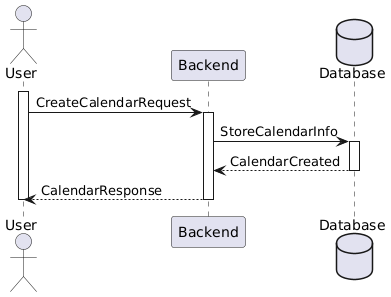
\includegraphics[width=0.5\textwidth]{images/docs/diagrams/sequence-diagrams/all-sequence-diagrams/Create Calendar.png}
  \caption{Create Calendar Sequence Diagram}
  \label{fig:seq/create-calendar}
\end{figure}

The ``Create Calendar Sequence Diagram'', shown in \textbf{Figure~\ref{fig:seq/create-calendar}}, illustrates the straightforward process of creating a new calendar within Jadwal. The sequence begins when the user initiates a CreateCalendarRequest gRPC call to the Backend, providing essential calendar details such as name and color preferences.

The Backend processes this request by executing a StoreCalendarInfo operation with the Database, which creates a new calendar record associated with the user's account. Upon successful storage, the Database confirms the creation with a CalendarCreated response. The Backend then sends a CalendarResponse back to the user through the gRPC channel, completing the calendar creation process.

This streamlined sequence ensures efficient calendar creation while maintaining data consistency. The process is designed to be quick and reliable, with proper error handling for network issues or database failures, allowing users to organize their schedules effectively within the Jadwal ecosystem.